%%%%%%%%%%%%%%%%%%%%%%%%%%%%%%%%%%%%%%%%%%%%%%%%%%%%%%%%%%%%%%%%%%%%
%% I, the copyright holder of this work, release this work into the
%% public domain. This applies worldwide. In some countries this may
%% not be legally possible; if so: I grant anyone the right to use
%% this work for any purpose, without any conditions, unless such
%% conditions are required by law.
%%%%%%%%%%%%%%%%%%%%%%%%%%%%%%%%%%%%%%%%%%%%%%%%%%%%%%%%%%%%%%%%%%%%

\documentclass[
  digital,     %% The `digital` option enables the default options for the
               %% digital version of a document. Replace with `printed`
               %% to enable the default options for the printed version
               %% of a document.
%%  color,       %% Uncomment these lines (by removing the %% at the
%%               %% beginning) to use color in the printed version of your
%%               %% document
  oneside,     %% The `oneside` option enables one-sided typesetting,
               %% which is preferred if you are only going to submit a
               %% digital version of your thesis. Replace with `twoside`
               %% for double-sided typesetting if you are planning to
               %% also print your thesis. For double-sided typesetting,
               %% use at least 120 g/m² paper to prevent show-through.
  nosansbold,  %% The `nosansbold` option prevents the use of the
               %% sans-serif type face for bold text. Replace with
               %% `sansbold` to use sans-serif type face for bold text.
  nocolorbold, %% The `nocolorbold` option disables the usage of the
               %% blue color for bold text, instead using black. Replace
               %% with `colorbold` to use blue for bold text.
  lof,         %% The `lof` option prints the List of Figures. Replace
               %% with `nolof` to hide the List of Figures.
  lot,         %% The `lot` option prints the List of Tables. Replace
               %% with `nolot` to hide the List of Tables.
]{fithesis4}
%% The following section sets up the locales used in the thesis.
\thesissetup{
    date        = \the\year/\the\month/\the\day,
    university  = mu,
    faculty     = fi,
    type        = bc,
    department  = Department of Machine Learning and Data Processing,
    author      = Dominik Rehák,
    gender      = m,
    advisor     = {RNDr. Vít Novotný, Ph.D.},
    title       = {Generic TeX Writer for the Pandoc Document Converter},
    TeXtitle    = {Generic \TeX{} Writer for the Pandoc Document Converter},
    keywords    = {LaTeX, Lua, Markdown, Pandoc, TeX, text analysis and parsing},
    TeXkeywords = {\LaTeX{}, Lua, Markdown, Pandoc, \TeX{}, text analysis and parsing},
    abstract    = {%
      This is the abstract of my thesis, which can

      span multiple paragraphs.
    },
    thanks      = {%
      These are the acknowledgements for my thesis, which can

      span multiple paragraphs.
    },
    bib         = bibliography.bib,
    %% Remove the following line to use the JVS 2018 faculty logo.
    facultyLogo = fithesis-fi,
}
\usepackage{makeidx}      %% The `makeidx` package contains
\makeindex                %% helper commands for index typesetting.
\usepackage[acronym]{glossaries}          %% The `glossaries` package
\renewcommand*\glspostdescription{\hfill} %% contains helper commands
\loadglsentries{terms-abbrs.tex}          %% for typesetting glossaries
\makenoidxglossaries                      %% and lists of abbreviations.
%% These additional packages are used within the document:
\usepackage{paralist} %% Compact list environments
\usepackage{amsmath}  %% Mathematics
\usepackage{amsthm}
\usepackage{amsfonts}
\usepackage{url}      %% Hyperlinks
\usepackage{markdown} %% Lightweight markup
\usepackage{multicol}
\usepackage{tikz}
\usetikzlibrary{positioning}
\usepackage{listings} %% Source code highlighting
\lstset{
  basicstyle      = \ttfamily,
  identifierstyle = \color{black},
  keywordstyle    = \color{blue},
  keywordstyle    = {[2]\color{cyan}},
  keywordstyle    = {[3]\color{olive}},
  stringstyle     = \color{teal},
  commentstyle    = \itshape\color{magenta},
  breaklines      = true,
  columns         = fullflexible,
}
\usepackage{floatrow} %% Putting captions above tables
\floatsetup[table]{capposition=top}
% \usepackage[babel]{csquotes} %% Context-sensitive quotation marks
\usepackage{pdfpages}
\usepackage{graphicx}
\usepackage[export]{adjustbox}

\usepackage{microtype}
\hyphenation{light-weight}
\hyphenation{con-struc-tors}

\let\oldlooseness=\looseness
\newcommand{\macro}[1]{\texttt{\textbackslash{}{#1}}}
\newcommand{\renderer}[1]{\texttt{\textbackslash{}markdownRenderer{#1}}}

\begin{document}
%% Uncomment the following lines (by removing the %% at the beginning)
%% and to print out List of Abbreviations and/or Glossary in your
%% document. Titles for these tables can be changed by replacing the
%% titles `Abbreviations` and `Glossary`, respectively.
%% \clearpage
%% \printnoidxglossary[title={Abbreviations}, type=\acronymtype]
%% \printnoidxglossary[title={Glossary}]

\chapter{Introduction}
\emph{Outline the goals of my thesis and the motivations behind them.}

\chapter{State of the art}
This chapter briefly introduces Pandoc and the relevant parts of its architecture. It also introduces the \TeX{} and \LaTeX{} typesetting systems and finally the Markdown package, which works with both of these systems and which will be utilized to quickly produce a simple proof of concept for the Pandoc writer.

\section{Pandoc}
\emph{Pandoc}~\cite{pandoc} is a utility which can convert between dozens of markup and document formats, such as HTML, docx, various Markdown flavours, some \TeX{} formats (e.g. \LaTeX{} and Con\TeX{}t), or roff macros for Unix manual pages. Pandoc consists of a core library written in the Haskell language and a command line tool providing access to this library.

Internally, the conversion in Pandoc is performed in two phases. First, the input format is converted into a native represenation, also called an \emph{abstract syntax tree} (or AST for short). Then, this AST is converted into the output format. Such a design allows for the input format readers to be written as modules independent of individual output format writers, and vice versa. This also makes it easy to extend the set of Pandoc's supported formats.

It should be noted that a support for a particular format does not have to be bidirectional. For example, Pandoc currently provides a Con\TeX{}t writer, but not a Con\TeX{}t reader. Thus, it is possible to implement a reader without a corresponding writer, and vice versa.

The AST itself is exposed via a special format named \texttt{native}, which inputs and outputs the entire AST in Pandoc's internal Haskell representaion. Alternatively, the format \texttt{json} inputs and outputs the AST in the JSON format.

\subsection{Usage}

The simplest way to use Pandoc is through the provided command line utility. When no arguments are provided, Pandoc takes text formatted with the Markdown markup language from standard input and outputs the HTML equivalent on the standard output:

$ $

\noindent
\begin{lstlisting}
$ echo 'Hello *world*!' | pandoc
<p>Hello <em>world</em>!</p>
\end{lstlisting}

$ $

Other builtin formats for input and output can be specificied using the \texttt{-{}-from} and \texttt{-{}-to} options (\texttt{-f} and \texttt{-t} for short). Naturally, one can also specify names of the input (argument without an option) and output (\texttt{-{}-output} or \texttt{-o}) files. For example, suppose we have the input file \textit{shopping-list.html} formatted using HTML with the following contents:

$ $

\noindent
\lstset{language=HTML}
\begin{lstlisting}
<h3>Shopping list</h3>
<ul>
    <li>Eggs</li>
    <li>Onions</li>
    <li>Butter</li>
    <li>Bread</li>
</ul>
\end{lstlisting}

$ $

\noindent
Then, the following command will the output file \textit{shopping-list.1} formatted using macros of the \textit{roff} typesetting system used for Unix manual pages:

$ $

\noindent
\lstset{language=}
\begin{lstlisting}
pandoc -f html -t man shopping-list.html -o shopping-list.1
\end{lstlisting}

$ $

\noindent
The contents of the output file \textit{shopping-list.1} will be:

$ $

\noindent
\begin{lstlisting}
.SS Shopping list
.IP \[bu] 2
Eggs
.IP \[bu] 2
Onions
.IP \[bu] 2
Butter
\end{lstlisting}
% \] % vim: stop highlighting an equation

$ $

If we want to define our own input/output format, we ultimately have two options. The first one is to directly extend the code of Pandoc itself with a new reader/writer module. This would require at least working knowledge Pandoc's codebase, as well as Haskell. Moreover, such a solution would not be very portable, as to actually use such a module, it would be necessary to recompile Pandoc. Of course, there is the possibility that Pandoc maintainers would consider the module worthy enough and of a sufficient quality (and the format significant enough) to include it into Pandoc itself. Even then, the format would only be available in new versions of Pandoc.

The other option is to write a reader/writer in the Lua programming language using the supported Lua API, which is described in Pandoc's documentation\footnote{\url{https://pandoc.org/custom-writers.html}}. Then, if we simply use the path to the Lua reader/writer as an input/output format, Pandoc's built-in Lua interpreter will parse and use that reader/writer at runtime. For example, if we defined a plain \TeX{} writer in the file \texttt{plaintex.lua} and then wanted to use plain \TeX{} as the output format, it would be enough to call:

$ $

\noindent
\begin{lstlisting}
$ echo 'Hello *world*!' | pandoc -t plaintex.lua
\end{lstlisting}

$ $

We will construct such a writer in Chapter 3.

$ $

As an aside, for some output formats (like \LaTeX{}, HTML or roff macros above), the default output produced by Pandoc does not constitute a complete document ready for viewing/typesetting, but rather just a short snippet. This can be amended by the \texttt{-{}-standalone} option (\texttt{-s}~for short), which surrounds the snippet with a template containing the skeleton of a full document. (Most of the templates are too long to reasonably embed an example of such an output here.)

\section{\TeX{}}
\TeX{} is a typesetting system designed and released by Donald Knuth in 1978. One of the main motivations for the creation of \TeX{} was the difficulty surrounding typesetting of mathematics at the time of its inception. \textit{(something else?)}

The input files of \TeX{} are plain text and their main elements are text to be typeset and control sequences, which influence how the text is to be typeset. 
Control sequences begin with their identifier, which consists of a backslash and a sequence of letters (uppercase or lowercase). Additionally, some control sequences take one or more of following tokens as parameters. The \TeX{} engine itself has around 300 of built-in control sequences, so-called \textit{primitives}.

An example of a primitive is \macro{end}, which is used for halting the \TeX{} engine and which takes no parameters. Another example is the primitive \macro{kern}, which inserts a blank fill of a given length. When the \TeX{} engine encounters \texttt{\textbackslash{}kern1em}, it inserts a blank fill, which is 1em wide.

Besides primitives, there can also be \textit{macros}, which are control sequences that recursively expand into other control sequences and groups of characters. Macros can be defined using the sequence \macro{def}, which can happen directly in the input file, or in a \textit{format}, which is essentially a collection of definitions in a single file. Knuth himself has defined such a format called \textit{plain \TeX{}} as the default format for \TeX{}.

An example of a macro is \macro{quad}, which is defined in plain \TeX{} as follows:

\noindent
\begin{lstlisting}
\def\enspace{\kern.5em}
\end{lstlisting}

When the macro is defined (e.g. by loading the format) and \macro{quad} is encountered by the \TeX{} engine, it is expanded into \texttt{\textbackslash{}kern.5em}. This results in a 0.5em wide blank fill as outlined above.

Several formats have been created specifically to provide abstractions above plain \TeX{} that allow greater focus on content rather than formatting itself, since plain \TeX{} can be cumbersome for creating documents. The most popular such system is \LaTeX{}, first released in 1984.

There exist multiple compatible implementations of the \TeX{} engine, some of which also implement their own primitives. An example is pdf\TeX{}, which is capable of direct output to PDF and also provides primitives for micro-typography. Another example is Lua\TeX{}, which will be of interest in chapter 3, since it is able to directly execute code written in the Lua language.

\section{The Markdown package for \TeX{}}
The \emph{Markdown}~\cite{cstug-markdown} \TeX{} package was named after Markdown, a lightweight markup language, which was first released in 2004 and designed with the primary goal of being easy to read and write. This has eventually caused wide adoption of the language on the Internet. The Markdown package provides a way to embed blocks of text written in the Markdown language directly into \TeX{} documents. During typesetting, these blocks are parsed and eventually expanded into native \TeX{} macros correspoding to the input. 

Because the Markdown package offers first-class support for plain \TeX{} and already tackles the task of converting high-level Markdown elements into low-level \TeX{} macros, it was suitable for its use in a working prototype of the plain \TeX{} writer for Pandoc. That is, the writer can simply produce macros defined by the Markdown package, which can then be expanded into \TeX{} primitives.

Regarding usage, the main intended way to use the Markdown package with plain \TeX{} is either through the macro \macro{markdownInput}, which is analogous to the \macro{input} primitive and takes a filename as an argument, or the pair of macros \macro{markdownBegin} and \macro{markdownEnd}, which surround a block of Markdown-formatted text directly embedded into the document source. Since we are mainly interested in the underlying macros that concern the individual Markdown element types, the thesis will not mention these macros further.

\subsection{Lunamark writer -- a previously explored approach}
Markdown's parser originates from a Lua library called \emph{Lunamark}~\cite{lunamark}, which is coincidentally also developed by John MacFarlane, the author of Pandoc. Lunamark provides a fast conversion of Markdown (its only input format) into other commonly used markup formats. Since the Lua\TeX{} engine is able to directly execute Lua code, Lunamark's parser was suitable for its use in the Markdown package.

\textit{(reformulate, describe this as a standalone project)} Here it should be noted that the original goal of the thesis was to integrate the support for Pandoc into the Markdown package. Such support allows users to embed blocks of all input formats, that are supported by Pandoc, into \TeX{} documents. This would be done by extending Lunamark with a reader module for Pandoc's AST (specifically the \texttt{json} format) and this support would then be transferred to the Markdown package. A prototype of this reader was actually written\footnote{\url{https://github.com/drehak/lunamark}}, before we \textbf{\textit{(who is we? Should I actually mention my supervisor here?)}} discovered that Pandoc supports external writers. The Lunamark writer was subsequently rewritten as a Pandoc writer, which outputs Markdown's macros, with a shim layer on top. (The details of this are all described in chapter 3). Eventually, it became clear that it is not necessary to extend Markdown with support for Pandoc, and that the macros introduced in what is now the proof of concept for the Pandoc writer could form a standalone package. At that point, the goal of the thesis had to be entirely reformulated.

\section{Comparison of Pandoc and Markdown}

\begin{itemize}
\item they kinda do the same thing
\item common elements
\item elements that work differently
\item elements without equivalents in Markdown
\end{itemize}

Elements of Pandoc's AST are somewhat similar to Markdown's macros for elements. Some of them are simple enough that it is possible to pass their contents to the corresponding macro -- that is, if they even have any.

An example of such an element would be \texttt{Emph}, which directly corresponds to the macro \renderer{Emphasis}. There is a few more elements with such equivalents, although in the case of \texttt{CodeBlock}, the order of its two parameters needs to be swapped:

\begin{itemize}
\item \texttt{Emph} $\rightarrow$ \renderer{Emphasis}
\item \texttt{Strong} $\rightarrow$ \renderer{StrongEmphasis}
\item \texttt{HorizontalRule} $\rightarrow$ \renderer{HorizontalRule}
\item \texttt{LineBreak} $\rightarrow$ \renderer{LineBreak}
\item \texttt{Note} $\rightarrow$ \renderer{Footnote}
\item \texttt{Code} $\rightarrow$ \renderer{CodeSpan}
\item \texttt{CodeBlock} $\rightarrow$ \renderer{InputFencedCode}
\end{itemize}

For other elements, the mapping to Markdown's macros is a bit more complicated. \emph{(TODO)}

Some Pandoc elements take a parameter of a type with multiple constant constructors. (In imperative languages, the closest equivalent would be an enumerable type.) For example, one of the parameters of \texttt{Cite} is of the type \texttt{CitationMode}, which itself has three constructors without parameters - \texttt{AuthorInText}, \texttt{SuppressAuthor} and \texttt{NormalCitation}. Another example would be \texttt{MathType} passed as a parameter of \texttt{Math} with two constructors, \texttt{DisplayMath} and \texttt{InlineMath}\footnote{In this case, the API for custom Pandoc writers splits handling of \texttt{Math} into two functions, \texttt{InlineMath} and \texttt{DisplayMath}. Depending on the value of \texttt{MathType}, Pandoc simply calls one of these two functions.}. Similarly, \texttt{Quoted} has a parameter \texttt{QuoteType} with two constructors, \texttt{SingleQuote} and \texttt{DoubleQuote}\footnote{Again, \texttt{Quoted} the API splits into two functions -- \texttt{SingleQuote} and \texttt{DoubleQuote}.} -- although \texttt{Quoted} has no equivalent among Markdown's macros.

Other elements are simply represented differently in Markdown. For example, the element \texttt{Header} contains its contents and an integer representing its level. (This maps nicely to the HTML tags \texttt{<h1>} to \texttt{<h6>}.) Markdown represents this using six individual macros, \renderer{HeadingOne} to \renderer{HeadingSix}.

\emph{(TODO - more?)}

Finally, there is a group of elements without any corresponding macros, like the afforementioned \texttt{Quoted}. This is understandable, since the syntax of Markdown does not cover these types of elements. A few more trivial examples would be \texttt{Underline}, \texttt{Strikeout}, \texttt{Superscript}, \texttt{Subscript} and \texttt{SmallCaps}. \emph{(TODO: Revise for latest Markdown version ($\rightarrow$ Future work))}

\begin{figure}
  \centering
  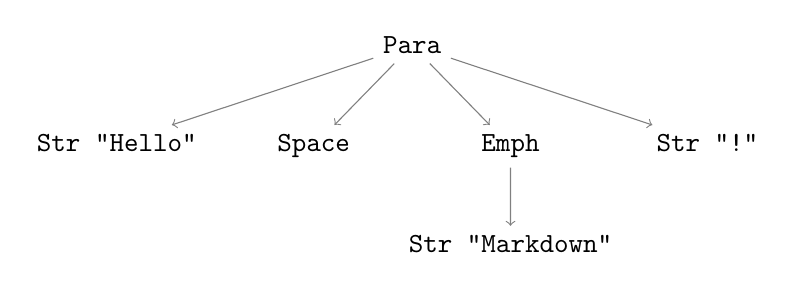
\begin{tikzpicture}[->, anchor=base, baseline, sibling distance=2.5cm, level distance=1.35cm]
    \node (pdpara) {\texttt{Para}}
      child { node (pdstrhello) {\texttt{Str "Hello"}} edge from parent[->, gray] }
      child { node (pdspace) {\texttt{Space}} edge from parent[->, gray] }
      child { node (pdemph) {\texttt{Emph}}
        child { node (pdstrmd) {\texttt{Str "Markdown"}} edge from parent[->, gray] }
      edge from parent[->, gray] }
      child { node (exclamation) {\texttt{Str "!"}} edge from parent[->, gray]
    };
  \end{tikzpicture}
  \caption{A graphical representation of Pandoc's AST for the Markdown input ``\texttt{Hello *Markdown*!}''}
  \label{fig:pandoc-ast}
\end{figure}

\begin{figure}
  \centering
  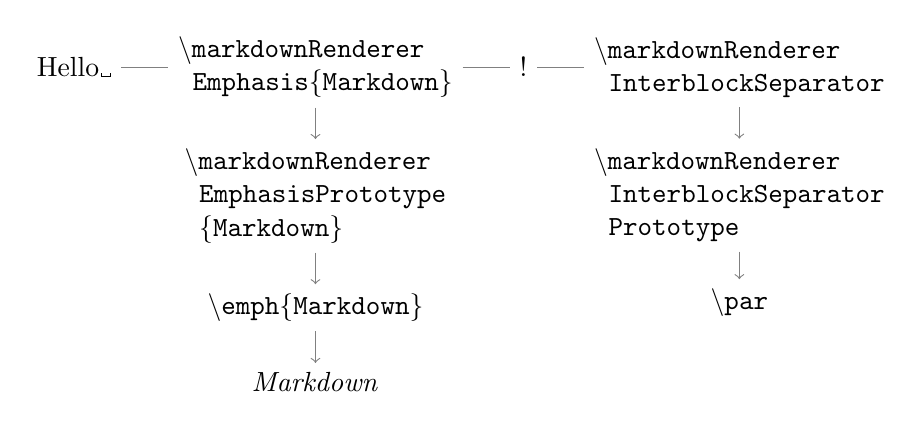
\begin{tikzpicture}[anchor=base, baseline, node distance=0.4cm]
    \node (hello) {Hello\textvisiblespace};
    \node [right=of hello, align=left, xshift=0.2cm] (mdemph) {
      \macro{markdownRenderer} \\
      \texttt{ Emphasis\{Markdown\}}
    } ;
      \node [below=of mdemph, align=left] (mdprotoemph) {
        \macro{markdownRenderer} \\
        \texttt{ EmphasisPrototype} \\
        \texttt{ \{Markdown\}}
      } ;
      \node [below=of mdprotoemph] (texemph) {\macro{emph\{Markdown\}}} ;
      \node [below=of texemph] (emph) {\emph{Markdown}} ;
    \node [right=of mdemph, xshift=0.2cm] (exclamation) {!} ;
    \node [right=of exclamation, align=left, xshift=0.2cm] (mdsep) {
      \macro{markdownRenderer} \\
      \texttt{ InterblockSeparator}
    } ;
      \node [below=of mdsep, align=left] (mdprotosep) {
        \macro{markdownRenderer} \\
        \texttt{ InterblockSeparator} \\
        \texttt{ Prototype}
      } ;
      \node [below=of mdprotosep, yshift=0.14em] (texsep) {\macro{par}} ;

    \path [gray] (hello) edge (mdemph) ;
      \path [gray, ->] (mdemph) edge (mdprotoemph) ;
      \path [gray, ->] (mdprotoemph) edge (texemph) ;
      \path [gray, ->] (texemph) edge (emph) ;
    \path [gray] (mdemph) edge (exclamation) ;
    \path [gray] (exclamation) edge (mdsep) ;
      \path [gray, ->] (mdsep) edge (mdprotosep) ;
      \path [gray, ->] (mdprotosep) edge (texsep) ;
  \end{tikzpicture}
  \caption{A graphical representation of macros generated by the Markdown package for the input ``\texttt{Hello *Markdown*!}''}
  \label{fig:markdown-ast}
\end{figure}

% Prvky Pandocu prevzaté z dokumentácie: \textsf{https://hackage.haskell.org/package/pandoc-types-1.22/docs/Text-Pandoc-Definition.html}

\begin{figure}
  \centering
  \begin{multicols}{3}
    \begin{compactenum}
      \item \texttt{Plain}
      \item \texttt{Para}
      \item \texttt{LineBlock}
      \item \texttt{CodeBlock}
      \item \texttt{RawBlock}
      \item \texttt{BlockQuote}
      \item \texttt{OrderedList}
      \item \texttt{BulletList}
      \item \texttt{DefinitionList}
      \item \texttt{Header}
      \item \texttt{HorizontalRule}
      \item \texttt{Table}
      \item \texttt{Div}
      \item \texttt{Null}
      \item \texttt{Str}
      \item \texttt{Emph}
      \item \texttt{Underline}
      \item \texttt{Strong}
      \item \texttt{Strikeout}
      \item \texttt{Superscript}
      \item \texttt{Subscript}
      \item \texttt{SmallCaps}
      \item \texttt{Quoted}
      \item \texttt{Cite}
      \item \texttt{Code}
      \item \texttt{Space}
      \item \texttt{SoftBreak}
      \item \texttt{LineBreak}
      \item \texttt{Math}
      \item \texttt{RawInline}
      \item \texttt{Link}
      \item \texttt{Image}
      \item \texttt{Note}
      \item \texttt{Span}
    \end{compactenum}
  \end{multicols}
  \vspace*{-1em}
  \caption{Complete list of elements of Pandoc's AST (as of Pandoc~2.14.2)}
  \label{fig:pandoc-elems}
\end{figure}

\begin{figure}
  \centering
  \begin{multicols}{2}
    \footnotesize
    \begin{compactenum}
      \item Tickbox Renderers
      \begin{compactenum}
        \item \texttt{TickedBox}
        \item \texttt{HalfTickedBox}
        \item \texttt{UntickedBox}
      \end{compactenum}
      \item \texttt{InterblockSeparator}
      \item \texttt{LineBreak}
      \item \texttt{Ellipsis}
      \item \texttt{Nbsp}
      \item Special Character Renderers
      \begin{compactenum}
        \item \texttt{Ampersand}
        \item \texttt{Backslash}
        \item \texttt{Circumflex}
        \item \texttt{DollarSign}
        \item \texttt{Hash}
        \item \texttt{LeftBrace}
        \item \texttt{PercentSign}
        \item \texttt{Pipe}
        \item \texttt{RightBrace}
        \item \texttt{Tilde}
        \item \texttt{Underscore}
      \end{compactenum}
      \item \texttt{CodeSpan}
      \item \texttt{Link}
      \item \texttt{Image}
      \item \texttt{ContentBlock}
      \item Bullet List
      \begin{compactenum}
        \item \texttt{UlBegin}
        \item \texttt{UlBeginTight}
        \item \texttt{UlItem}
        \item \texttt{UlItemEnd}
        \item \texttt{UlEnd}
        \item \texttt{UlEndTight}
      \end{compactenum}
      \item Ordered List
      \begin{compactenum}
        \item \texttt{OlBegin}
        \item \texttt{OlBeginTight}
        \item \texttt{OlItem}
        \item \texttt{OlItemEnd}
        \item \texttt{OlItemWithNumber}
        \item \texttt{OlEnd}
        \item \texttt{OlEndTight}
      \end{compactenum}
      \item Definition List
      \begin{compactenum}
        \item \texttt{DlBegin}
        \item \texttt{DlBeginTight}
        \item \texttt{DlItem}
        \item \texttt{DlItemEnd}
        \item \texttt{DlDefinitionBegin}
        \item \texttt{DlDefinitionEnd}
        \item \texttt{DlEnd}
        \item \texttt{DlEndTight}
      \end{compactenum}
      \item Emphasis
      \begin{compactenum}
        \item \texttt{Emphasis}
        \item \texttt{StrongEmphasis}
      \end{compactenum}
      \item Block Quote
      \begin{compactenum}
        \item \texttt{BlockQuoteBegin}
        \item \texttt{BlockQuoteEnd}
      \end{compactenum}
      \item Code Block
      \begin{compactenum}
        \item \texttt{InputVerbatim}
        \item \texttt{InputFencedCode}
      \end{compactenum}
      \item YAML Metadata
      \begin{compactenum}  % nepotrebné?
        \item \texttt{JekyllDataBegin}
        \item \texttt{JekyllDataEnd}
        \item \texttt{JekyllDataMappingBegin}
        \item \texttt{JekyllDataMappingEnd}
        \item \texttt{JekyllDataSequenceBegin}
        \item \texttt{JekyllDataSequenceEnd}
        \item \texttt{JekyllDataBoolean}
        \item \texttt{JekyllDataNumber}
        \item \texttt{JekyllDataString}
        \item \texttt{JekyllDataEmpty}
      \end{compactenum}
      \item Heading
      \begin{compactenum}
        \item \texttt{HeadingOne}
        \item \texttt{HeadingTwo}
        \item \texttt{HeadingThree}
        \item \texttt{HeadingFour}
        \item \texttt{HeadingFive}
        \item \texttt{HeadingSix}
      \end{compactenum}
      \item \texttt{HorizontalRule}
      \item \texttt{Footnote}
      \item \texttt{Cite}
      \item \texttt{TextCite}
      \item \texttt{Table}
      \item \texttt{InlineHtmlComment}
    \end{compactenum}
  \end{multicols}
  \vspace*{-1em}
  \caption{A complete list of output macros of the Markdown package for version 2.11.0}
  \label{fig:markdown-renderers}
\end{figure}

\chapter{Implementation}
In this chapter, I will describe how the proof of concept for the plain \TeX{} writer for Pandoc was implemented. Additionally, I will demonstrate the usage of the writer on a set of example documents.

\section{The custom Pandoc writer itself}
As described in chapter 2, a custom Pandoc writer consists of a single file written in Lua. The Pandoc documentation provides a sample custom writer for HTML and recommends using this writer as a basis for other custom writers, which is what I did. I will refer to this modified file as \texttt{pandoc-to-markdown.lua}, which is also its name in the proof of concept.

For each AST element type, the writer defines a pure function that outputs the element in the output format. If the element has any child elements, they have already been processed by other functions by the time they are passed as arguments. Therefore, it is not necessary to implement the recursive descent manually.

Functions in \texttt{pandoc-to-markdown.lua} return macros of the form \macro{pandocElementName}, similarly to the Markdown package with its \renderer{ElementName}. These macros are defined in the \texttt{pandoc-to-markdown.tex} file. This allows the user to change the appearance of elements by simply redefining the macros on the \TeX{} side.\footnote{The proof of concept actually uses this in \texttt{pandoc-to-markdown.sty} to redefine some macros with equivalent \LaTeX{} constructs.} It also results in a somewhat cleaner implementation, since the style of all elements is defined in a single \TeX{} file. \textit{(reformulate?)}

Internally, Pandoc splits elements into two groups of inline elements and block elements. As the name suggets, block elements appear as vertically separate blocks in the document (e.g. paragraphs, lists or tables), while inline elements can occur inside a line of text - which is generally a block element. This distinction does not matter for the user, perhaps not even the author of a custom writer. However, it constrains which elements can appear in others - for each child element, it is specified whether it's a block element or an inline element. Generally, block elements can contain block elements or inline elements, while inline elements can only contain other inline elements.\footnote{The one exception to this is \texttt{Note}, which represents a footnote or an endnote and its contents are represented as a list of block elements. However, these elements appear outside the parent element of the note, such as the contents of this footnote.}

I have reordered the functions in \texttt{pandoc-to-markdown.lua} so that they appear in the same order in which they are defined in Pandoc\footnote{\url{https://hackage.haskell.org/package/pandoc-types-1.22/docs/Text-Pandoc-Definition.html}}. Nevertheless, since inline elements are structurally simpler and cannot contain block elements, I will describe them first.

\subsection{Inline elements}

The first inline element is \texttt{Str}, which simply defines a string without spaces. A trivial example of this can be seen in figure \ref{fig:html-browsers-typeset}. To provide correct \TeX{} output, it will be necessary to escape characters that have a special role in \TeX{}. Since the Markdown package already provides macros for these characters, for example \renderer{Backslash}, the occurences of these characters will be replaced with their respective macros. (It is possible that letters will occur after the special characters, so braces are added after the macro name, e.g. \macro{pandocBackslash\{\}}. This does not affect the behavior of the macro, but it prevents the \TeX{} tokenizer from considering the letters as a part of the macro name.) The sample writer already provides an example function for escaping strings - for HTML, of course:

$ $

\noindent
\lstset{language=[5.3]Lua}
\begin{lstlisting}
local function escape(s, in_attribute)
  return s:gsub('[<>&"\']',
    function(x)
      if x == '<' then
        return '&lt;'
      elseif x == '>' then
        return '&gt;'
      elseif x == '&' then
        return '&amp;'
      elseif in_attribute and x == '"' then
        return '&quot;'
      elseif in_attribute and x == "'" then
        return '&#39;'
      else
        return x
      end
    end)
end
\end{lstlisting}

$ $

\noindent
There is a problem with this construct -- \texttt{gsub} replaces all occurences of the given characters in \texttt{s}. However, if the modified function for plain \TeX{} output would in this way replace \texttt{\{} with \texttt{\textbackslash{}pandocLeftBrace\{\}}, this would generate another occurence of \texttt{\{}, which would also get replaced with \texttt{\textbackslash{}pandocLeftBrace\{\}}\dots and so on. This can be mitigated by saving the substitution into a variable and returning it at the end of the inner function. (Some characters in the pattern provided to \texttt{gsub} have to be escaped with \%.)

$ $

\noindent
\lstset{language=[5.2]Lua}
\begin{lstlisting}
local function escape(s)
  s = string.gsub(s, "[\\{}%|_#&~%^%%%$]", function(c)
    local s
    if     c == "&"  then s = "\\pandocAmpersand{}"
    elseif c == "\\" then s = "\\pandocBackslash{}"
    elseif c == "^"  then s = "\\pandocCircumflex{}"
    elseif c == "$"  then s = "\\pandocDollarSign{}"
    elseif c == "#"  then s = "\\pandocHash{}"
    elseif c == "{"  then s = "\\pandocLeftBrace{}"
    elseif c == "%"  then s = "\\pandocPercentSign{}"
    elseif c == "|"  then s = "\\pandocPipe{}"
    elseif c == "}"  then s = "\\pandocRightBrace{}"
    elseif c == "~"  then s = "\\pandocTilde{}"
    elseif c == "_"  then s = "\\pandocUnderscore{}"
    else                  s = c
    end
    return s
  end)
  return s
end
\end{lstlisting}

$ $

\noindent
The function for \texttt{Str} itself is same as in the sample writer.

$ $

\noindent
\lstset{language=[5.2]Lua}
\begin{lstlisting}
function Str(s)
  return escape(s)
end
\end{lstlisting}

$ $

\noindent
Next inline element is \texttt{Emph}, representing emphasis. \texttt{Emph} contains a list of inline elements, but any special characters have already been escaped by \texttt{Str} executed on the strings inside, so there is no need to do that again. Here, the Lua operator \texttt{..} performs concatenation.

$ $

\noindent
\lstset{language=[5.3]Lua}
\begin{lstlisting}
function Emph(s)
  return "\\pandocEmph{" .. s .. "}"
end
\end{lstlisting}

$ $

\noindent
\macro{pandocEmph} is defined in \texttt{pandoc-to-markdown.tex}, as outlined above:

$ $

\noindent
\lstset{language=[plain]TeX}
\begin{lstlisting}
\def\pandocEmph{\markdownRendererEmphasis}%
\end{lstlisting}

$ $

\noindent
Next is \texttt{Underline}. The original Markdown language has no way to represent an underline, so there is no support for it in the Markdown package.\footnote{As of version 2.11.0.} For now, we will simply define a macro which expands to its parameter, rendering it as a plain string.

$ $

\noindent
\lstset{language=[5.3]Lua}
\begin{lstlisting}
function Underline(s)
  return "\\pandocUnderline{" .. s .. "}"
end
\end{lstlisting}

$ $

\noindent
\texttt{pandoc-to-markdown.tex}:

$ $

\noindent
\lstset{language=[plain]TeX}
\begin{lstlisting}
\def\pandocUnderline#1{#1}%
\end{lstlisting}

$ $

\noindent
For the next few inline elements, the structure of the writer functions is virtually the same, so it is not worth listing them here. The macros look similar too. The only new construct occurs in \macro{pandocSingleQuoted} and \macro{pandocDoubleQuoted}, which surround their parameter with \texttt{`} and \texttt{'}, the characters used by \TeX{} to represent quotes:

$ $

\noindent
\lstset{language=[plain]TeX}
\begin{lstlisting}
\def\pandocStrong{\markdownRendererStrongEmphasis}%
\def\pandocStrikeout#1{#1}%
\def\pandocSubscript#1{#1}%
\def\pandocSuperscript#1{#1}%
\def\pandocSmallCaps#1{#1}%
\def\pandocSingleQuoted#1{`#1'}%
\def\pandocDoubleQuoted#1{``#1''}%
\end{lstlisting}

$ $

% With \texttt{Cite}, things start to get a little bit complicated



\subsection{Block elements}

\subsection{Escaping special characters}

\section{\TeX{} macropackage surrounding the writer}
\emph{
This section will describe pandoc-to-markdown.tex, as well as pandoc-to-markdown.sty.
}

\subsection{pandoc... macros}
\emph{
Describe the set of macros that was implemented. Maybe it's worth it to also describe the \LaTeX{} overrides.
}

\subsection{Caveats}
\emph{maybe nějaký veselý historky z natáčení (shellesc/write18, pandocInput, jak pejsek s kočičkou spustili Pandoc z TeXu, codeBlocks v samostatných súboroch + auxdir (haha) etc.)}

\section{Example documents}
\emph{Demonstrate specific example documents and the problems they posed while implementing the writer. \label{fig:html-browsers-typeset} \textbf{Consider if this should not be a separate chapter.}}

% \includepdf[pages={1}]{pandoc-to-markdown/examples/html-browsers.pdf}

% \begin{figure}[h]
%    \centering
%    \begin{tabular}{@{}c@{\hspace{.5cm}}c@{}}
%      \includegraphics[
%        width=0.6\textwidth,
%        page=1,
%        frame,
%        trim=2cm 2cm 2cm 2cm
%      ]{pandoc-to-markdown/examples/html-browsers.pdf}
%    \end{tabular}
%  \caption{Example page from an \textsc{HTML} document typeset with the proof of concept}
%  \label{fig:html-browsers-typeset}
% \end{figure}

\chapter{Conclusion}
\section{Future work}
\emph{Mention open issues. Also the Haskell plans, solidification of the macros interface and the relevant ongoing discussion.}

\subsection{Handling of deprecation of classic custom writers}

There are currently two styles of defining custom writers for Pandoc, to which the Pandoc documentation refers to as ``classic'' and ``new''. The main difference between them is that the classic style writer defines its rendering functions on the top level, while in the new style, everything is processed through a top-level function named \texttt{Writer} which contains all the custom writer logic.

For the plain \TeX{} writer, I have decided to go with the classic style. There were multiple reasons for this, the main one being that the classic style is what Pandoc's documentation covers. Another reason is that support for the new style was only introduced in Pandoc 2.18\footnote{The Pandoc documentation actually states that the new style of custom writers was introduced in 2.17.2. This is wrong. No such version was even released, 2.17.1.1 was immediately followed by 2.18.}, which was released in January 2022. Repositories of several high-profile Linux distributions ship versions of Pandoc that are way older than that. For instance, Fedora 37 released in November 2022 provides only packages with Pandoc 2.14.0.3\footnote{\url{https://packages.fedoraproject.org/pkgs/pandoc/pandoc/fedora-37.html}}, which was released in June 2021. Another example is Ubuntu 22.04 LTS (codenamed ``Jammy Jellyfish''), which, despite being released in April 2022, still ships Pandoc 2.9.2.1\footnote{\url{https://packages.ubuntu.com/jammy/pandoc}} from March 2020.

Unbeknownst to me at the time, classic custom writers were going to be deprecated. According to the discussion on the related pull request\footnote{\url{https://github.com/jgm/pandoc/pull/8343}}, it will still be possible to update a classic writer to a new-style one. However, other breaking changes might still be introduced. As long as the plain \TeX{} writer is an external one instead of being built into Pandoc itself, it will have to deal with this in the future.

\printbibliography[heading=bibintoc] %% Print the bibliography.

\makeatletter\thesis@blocks@clear\makeatother
\phantomsection %% Print the index and insert it into the
\addcontentsline{toc}{chapter}{\indexname} %% table of contents.
\printindex

\appendix %% Start the appendices.
\chapter{An appendix}
Here you can insert the appendices of your thesis.

\end{document}
